\documentclass[10pt,a4paper]{article}
\usepackage[utf8]{inputenc}
\usepackage[english]{babel}
\usepackage[T1]{fontenc}
\usepackage{amsmath}
\usepackage{amsfonts}
\usepackage{amssymb}
\usepackage{subcaption}
\usepackage{makeidx}
\usepackage{graphicx}
\usepackage{fourier}
\usepackage{listings}
\usepackage{color}
\usepackage{hyperref}
\usepackage[left=2cm,right=2cm,top=2cm,bottom=2cm]{geometry}
\author{Tommy Müller, Marcus Dittrich, Vincent Noculak}
\title{Rastertunnelmikroskop}

\lstset{language=C++,
	keywordstyle=\bfseries\color{blue},
	commentstyle=\itshape\color{red},
	stringstyle=\color{green},
	identifierstyle=\bfseries,
	frame=single}
\begin{document}

\maketitle
\newpage
\tableofcontents
\newpage

\section{Vermessung von Graphit }

\subsection{ Kantenhöhen}

Mit dem Rastertunnelmikroskop haben wir 79 Bilder aufgenommen. Davon waren 16 zum Kantenvermessen geeignet.
Diese Bilder haben wir mit dem Tool WSxM 4.0 Beta 8.2 vermessen. 
Wir benutzen die Funktionen "Local plane" und "profile". "Local plane" reskaliert, nach Auswahl von ebenen Flächen, das gesamte Bild.  Die Funktion "profile" liefert ein Höhenprofil der Verbindungslinie zwischen zwei ausgewählten Punkten (Siehe Bilder der Kanten unten).
Viele Bilder waren fehlerhaft und konnten nicht zur Bestimmung von Kantenhöhen verwendet werden.
Ursachen dafür waren thermische Verschiebung (Drift), Creep, Bildfehler \ref{b12} oder keine verwertbare Kanten auf den Bildern. Wir haben jede Kante an 5 unterschiedlichen Orten vermessen, dies lieferte den Mittelwert und den Fehler als Standardabweichung.



\subsection{Beispiel Kanten}

\begin{figure}[]
	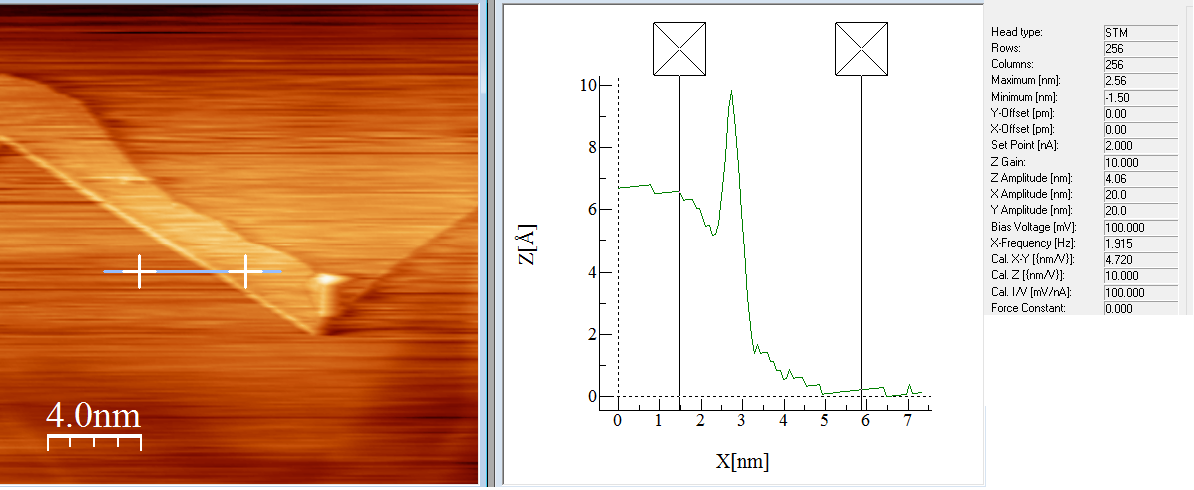
\includegraphics[scale = 0.3]{bild00.png}
	\centering
	\caption{Bild 0. Kante 0.637 nm und RTM Daten}
	\label{b0}
\end{figure}

\begin{figure}[]
	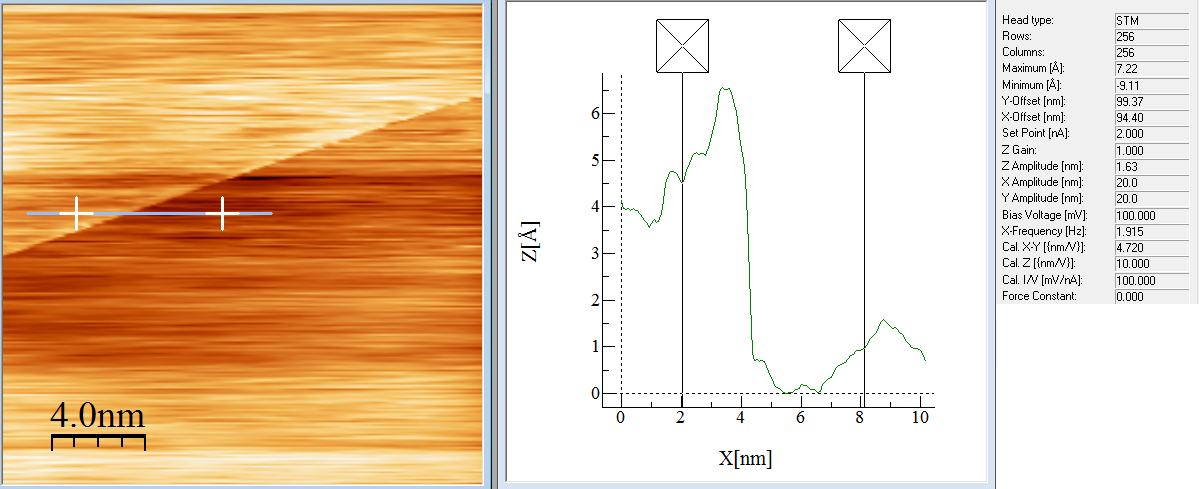
\includegraphics[scale = 0.3]{bild11.png}
	\centering
	\caption{Bild 11. Kante 0.353 nm und RTM Daten}
	\label{b11}
\end{figure}
\begin{figure}[]
	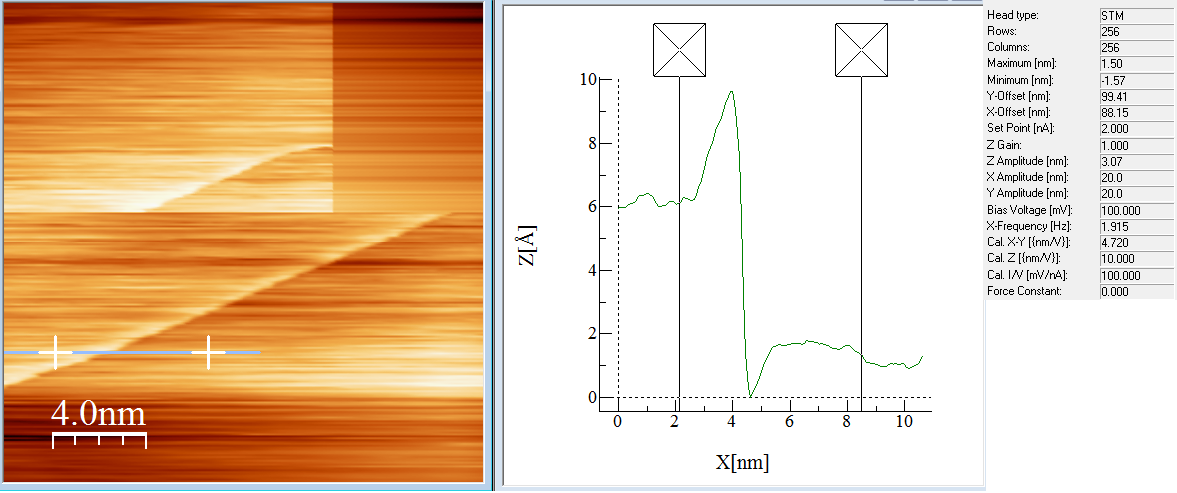
\includegraphics[scale = 0.3]{bild12.png}
	\centering
	\caption{Bild 12. Kante 0.447 nm und RTM Daten}
	\label{b12}
\end{figure}




In dem Diagramm \ref{kantendia} sind alle gemittelten Kanten eingetragen. Die Höhen gingen von 0.272  $ \pm 0.149 $ nm bis 1.893 $ \pm 0.250 $ nm. Die theoretischen Kanten wurden mit den roten Linien markiert.

\begin{figure}[]
	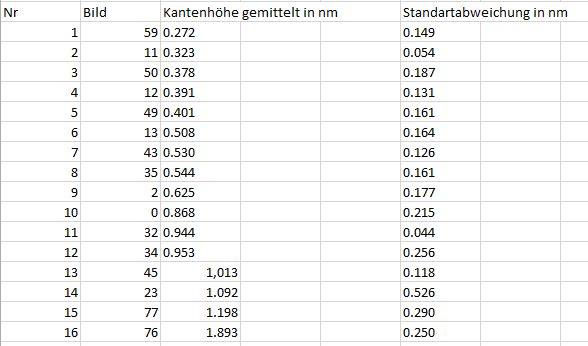
\includegraphics[scale = 0.5]{Kantengeordnetrichtig.png}
	\centering
	\caption{Liste der geordeneten Kanten}
	\label{list}
\end{figure}

\begin{figure}[]
	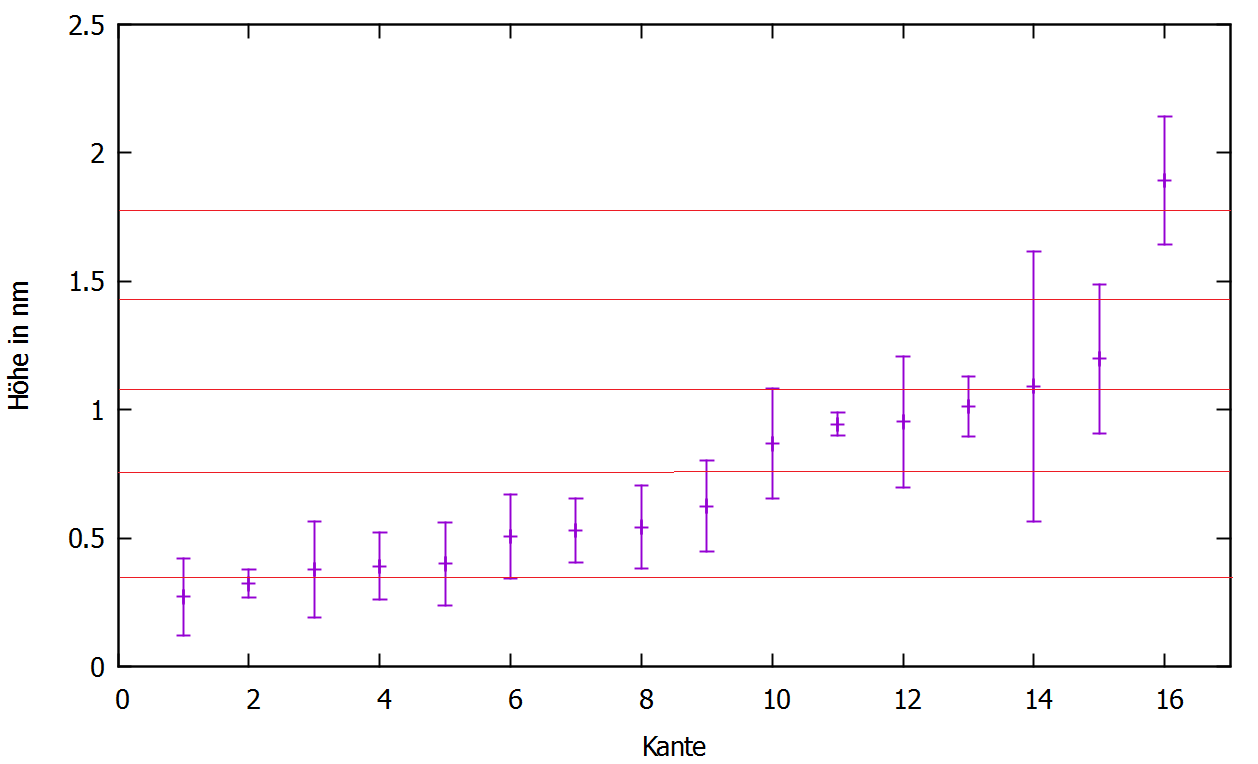
\includegraphics[scale = 0.5]{kantendiag.png}
	\centering
	\caption{Diagramm Höhe der Kanten sowie in Rot die theoretische Kantenhöhen}
	\label{kantendia}
\end{figure}

In dem Diagramm\ref{kantendia} sehen wir eine Ansammlung von Messwerten bei der erst- und dritten Kante. Diese Kanten werden deshalb am besten durch unsere Messungen repräsentiert. Die anderen theoretischen Kanten werden nur bedingt durch unsere Messergebnisse widergespiegelt.
Anhand des Graphen ordnen wir die ersten sechs Kanten der einfachen Gitterkonstante zu, da die Fehlerbalken über den theoretische Ebenenabstand geht. Kante 7 und 8 sind genau zwischen zwei theoretischen Kanten und danach wird die Zuordnung von Kante zu n-fachen der Gitterkonstante nicht einfacher.
Jede Kante wurde der n- fachen Ebenenabstand zugeordnet, dessen Mittelpunkt am nächsten der theoretischen Ebene war. Kante 7 und 8 wurden daher ausgelassen, da eine eindeutige Zuordnung nicht möglich war(genau zwischen zwei Gitterkonstanten). Unsere gemessene Gitterkonstante ist $(3.5 \pm 0.6) \mathring{A}$. Werte entstehen aus dem Mittelwert der durch n gewichteten Kanten und dessen Standardabweichung. \\ 
q =  $\frac {theo. Ebenenkosntante} {gemessene Ebenenkonstante}$\\
Der q- Wert ist wichtig für die Kalibrierung des Z - Piezos.
Gehen wir nun von der Kalibrierung des Z- Piezos mit 10 nm per Volt aus, müssen wir diesen Wert auf $10 \frac {nm} {v} * q = (9.5 \pm1.5)nm$ nach unten korrigieren.



\subsection{ Diskussion}

Beim Vergleichen der theoretischen Kanten mit dem Messergebissen muss drauf geachtet werden, dass die Kanten nicht durch Drift oder Creep unscharf werden, bzw. keine Kanten im Kristall sind. Die Form der Spitze ist entscheidend. Da diese mit einer Drahtschere gefertigt wurde(keine einatomige Spitze), sind größere Messfehler zu erwarten. Weitere Fehlerquellen sind die Ungenauigkeit und Inhomogenität des Piezos und die Graphitprobe selbst.
Mit unseren Messbildern konnten wir 16 Kanten an der Graphitoberfläche vermessen. Diese Kanten wurden nach der Höhe geordnet und in Diagramm \ref{kantendia} dargestellt. Wir konnten mit unseren Messergebnissen die theoretischen Kanten relativ schlecht darstellen. Vor allem den ersten und dritten Netzebenenabstand können unsere Messergebnisse rekonstruieren. Einige Messergebisse sind fast genau zwischen zwei Ebenen, dies könnte an der schlechten Wahl von Messpunkten in Messbildern liegen. Eine Vorsondierung der Bilder wäre von Nöten gewesen, um mehr Kanten zu erfassen und die Ergebnisse klarer zu gestalten.
Der von uns, mit dem Kantenhöhen bestimmte Ebenenabstand des Graphits ist $(3.53 0.58)\mathring{A}$ und damit im einfachen Fehlerintervall zum Literaturwert von 3.35 $\mathring{A}$, die nur dem großen Fehler unserer Messdaten zugrunde liegt. (Quelle: Anleitung zum Rastertunnelmikroskop, BA10 Fu Berlin Praktikum)

\end{document}